\chapter{}

Tomaz crescia forte e esperto.
Andou e falou antes de completar um ano.
Tínhamos alugado uma casa próxima à casa dos meus pais.
E eu logo me descobri grávida de novo.
Marcelo estava a caminho.
  

\begin{figure}
\centering
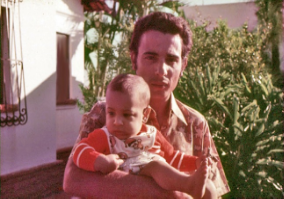
\includegraphics[width=0.8\linewidth]{25/de-volta.png}
\caption{De volta a Araraquara, com Tomaz.}
\end{figure}

\begin{figure}
\centering
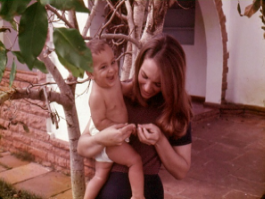
\includegraphics[width=0.8\linewidth]{25/tomaz.png}
\caption{Tomaz, aos oito meses.}
\end{figure}

\begin{figure}
\centering
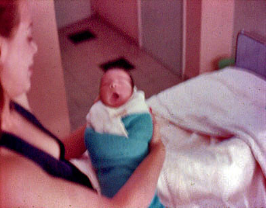
\includegraphics[width=0.8\linewidth]{25/marcelo-mundo.png}
\caption{Marcelo chegando ao mundo.}
\end{figure}

\begin{figure}
\centering
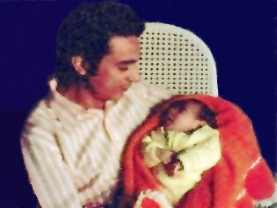
\includegraphics[width=0.8\linewidth]{25/no-colo.png}
\caption{Recém-nascido, no colo do pai.}
\end{figure}

Marcelo nasceu em 24 de maio de 1974.
Com jeitinho de japonês, cabelos pretos e lisos espetados para o alto, olhinhos apertados, nariz de batatinha.
Na verdade, sofreu uma espécie de despejo, a poder de citocina, porque dez dias se passaram da data aprazada e ele não demonstrava o menor interesse em deixar o ninho.
Minha sogra, aflita com a espera, chegou a bordar naqueles dias grande parte de uma tapeçaria que hoje enfeita a parede 
do escritório de casa.
Mas o bem-humorado garotinho não deu mostras de se aborrecer por ter sido desalojado daquela maneira.
Irradiava simpatia e não se abalou nem mesmo com a hostilidade momentânea do irmão mais velho.


D. Yolanda preparou Tomaz com sua melhor roupinha, penteou-lhe os cabelos com capricho e espetou-lhe nas mãos um ramo de flores, tudo para esperar a mim e ao irmãozinho que vínhamos chegando da maternidade.
No momento em que a porta se abriu e ele me viu trazendo Marcelo nos braços, atirou o ramalhete na minha direção, saiu correndo e foi refugiar-se emburrado e lacrimejante no cômodo mais distante da casa.
Sem conseguir demovê-lo, fui cuidar de organizar as coisas, enquanto o bebê dormia.
Horas mais tarde, Marcelo pôs-se a reclamar de fome.
Ao entrar no quarto, deparei-me com Tomaz estudando atentamente a criaturinha, tão entretido que nem percebeu minha chegada.
Escondi-me.
Marcelo começou a chorar.
Agoniado, Tomaz desandou a correr pela casa me chamando para acudir o irmão.
A partir daí, adotou-o.
Nunca o surpreendi num gesto agressivo.
Ao contrário, tomou-se de cuidados e pulava ao menor ruído vindo do berço.
Mas o irmãozinho passou a ser também o seu brinquedo preferido.
Assim que Marcelo começou a engatinhar, rolava com ele pelo chão como se o coitado fosse um bicho de pelúcia.
E o irmãozinho parecia achar aquilo muito divertido, porque ria a mais não poder.
Gosto de pensar que ali teve início a sólida amizade que os une até hoje.

\begin{figure}
\centering
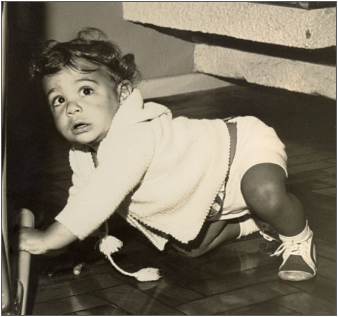
\includegraphics[width=0.7\linewidth]{25/marcelo-1o-ano.png}
\caption{Marcelo, no primeiro ano de vida.}
\end{figure}

\begin{figure}
\centering
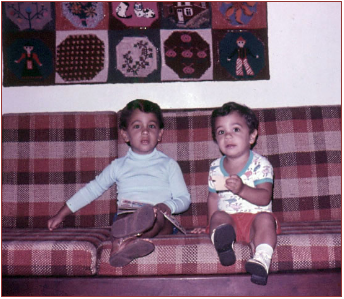
\includegraphics[width=0.7\linewidth]{25/tomaz+marcelo.png}
\caption{Tomaz e Marcelo em 1976.}
\end{figure}

A cada dia ficava mais evidente que a situação da fazenda era insustentável.
O café começava a granar, anunciando sua primeira e promissora safra, mas não havia mais onde buscar dinheiro.
Os sócios que Paulo arrumara na tentativa de salvar a Santa Teresa, foram desistindo, um a um.
A fazenda acabou sendo vendida.

O acerto com os colonos foi feito, os sócios foram pagos, a nossa parte ficou para o fim.
Em 1975, a temida ``geada negra'' abateu-se sobre o Paraná e o Mato Grosso, queimando até o toco o cafezal exuberante da Santa Teresa.
A fazenda já não nos pertencia, mas doeu pensar que de todo aquele esforço quase nada restara.
E mesmo o pouco dinheiro que constituía nossa parte do acerto, diante de toda aquela desgraça, teríamos de esperar muito para recebê-lo.

Agora morávamos num sobrado vizinho da fábrica do meu pai e eu estava grávida, de novo.
Com dois filhos nascidos e um terceiro a caminho, Paulo tivera que sair atrás de trabalho.
Para nosso alívio, prestou concurso para a Casa da Lavoura e foi aprovado entre os primeiros colocados.
Pôde escolher Tabatinga, uma cidade próxima de Araraquara.
Era um emprego público, o único, diziam, em que de fato se praticava agronomia, mas não pagava grande coisa.
Paulo complementava o salário fazendo fiscalização para bancos e projetos para obtenção de crédito agrícola.
Era um bocado sacrificado.
Eu continuava dando aulas e às vezes, à noite, grávida, cansada de subir e descer as escadas do sobrado, cuidando de fazer as mamadeiras e de pôr os meninos na cama, eu me aborrecia de vê-lo mergulhado naquele mar de formulários, sem erguer a cabeça um momento sequer.
Uma vez, estava eu às voltas com o ritual noturno de dar o banho coletivo, vestir pijamas, distribuir mamadeiras e cantar para niná-los, quando Paulo reclamou do barulho que o desconcentrava.
Retruquei, furiosa: 

\textit{``-- Sabia que Bach escreveu suas maiores obras-primas numa casa minúscula, rodeado por catorze filhos pequenos?''}

\textit{``-- Ah, bom''}, rebateu ele, \textit{''então vou ver se componho uma sinfonia, porque preencher relatório de fiscalização no meio dessa zoada, não dá, não!''}

Contudo, Fernando, nosso terceiro filho, pareceu nascer muito consciente da situação.
Não dava o menor trabalho, era auto-suficiente e compenetrado.
Aprendeu a subir as escadas sozinho assim que começou a engatinhar e quando o surpreendi andando, chorei.
Não me dera conta dos progressos que, sem alarde, ele fizera.
Felizmente, carinho era o que não lhe faltava.
Gordinho, cachinhos de anjo barroco, ia de colo em colo recebendo os dengos de avós, tias e primas sempre quietinho, contemplando aquele bando de adultos lhe fazendo gracinhas como se observasse macacos num zoológico.
Mas, gostava e aninhava-se entre a mulherada como cachorrinho novo oferecendo a barriguinha aos cafunés.

\begin{figure}
\centering
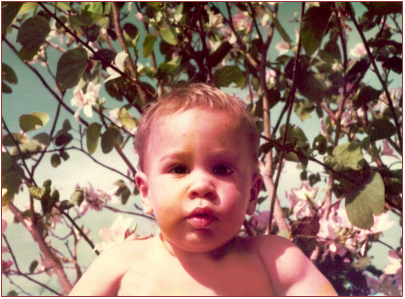
\includegraphics[width=0.8\linewidth]{25/fernando-bebe.png}
\caption{Fernando bebê.}
\end{figure}

\begin{figure}
\centering
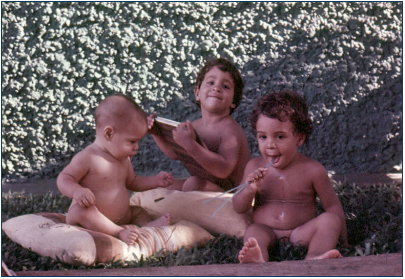
\includegraphics[width=0.8\linewidth]{25/irmãos.png}
\caption{Os irmãos brincando no jardim.}
\end{figure}
